\section{NumInt}
Verbesserung der Näherung: Aufteilung in kleine Teilintervalle \& Summe von Rechtecksflächen bilden; Interpolations mit Polynom höheren Gredes durch diskrete Punkte.
\subsection{Def}
$ p_{k} \hat{=} $ Interpolationspolynom; 
$ I_{n} \hat{=} $ Quadraturformel; 
$ K \hat{=} $ Fehlerkonstante des Verfahrens.; 
Singularität $\hat{=}$ isolierter Punkt, der ungewöhnliches Verhalten zeigt; 

\subsection{Newton-Cotes}
Das Intergral des $ p_{k} $ diens al Appr. für das Int. von f(x); 
$ \int_{0}^{1} f(t) dt \approx \int_{0}^{1} p_{k} (t) dt =  \sum_{j=0}^{k} \alpha_j f( t_{j} ) $ Das Interpolationspolynom muss nicht explizit aufgestellt werden, es dient vorab der Bestimmung der Gewichte $ \alpha_{j} $; 
$ \int_{0}^{1} p_{k}(t) = \int_{0}^{1} \sum f( t_{j} ) L_{j} (t) dt = \sum f ( t_{j} ) \int_{0}^{1} L_{j} (t) dt $
\subsubsection{Trapezregel}
$ T_{1}: $ 
$ \int_{0}^{1} f (t) dt \approx \frac{1}{2} ( f(0) + f(1) ) $; 
$ \int_{a}^{b} f (x) dx \approx \frac{(b-a)}{2} (f(a) + f(b) ) $;\\
$ T_{n}: $
Für Teilintervalle mit gleicher Länge: $ h = \frac{b-a}{n} $;  
$ T_{n} = h (\frac{ f ( x_{0} ) }{2} + f(x_{1}) + ... + f(x_{n-1}) + \frac{ f(x_n) }{2} ) $; 
\subsubsection{SimpsonRegel}
$ S_{1}: $ 
$ \int_{0}^{1} f (t) dt \approx \frac{1}{6} ( f(0) + 4f(0.5) + f(1) ) $; 
$\int_{a}^{b} f (x) dx \approx \frac{b-a}{6} ( f(a) + 4f( \frac{a+b}{2}) + f(b) ) $; 
Für n = 1: $\frac{( b-a )}{2\cdot1} \frac{1}{3} ( f(a) + 4f( \frac{a+b}{2}) + f(b) ) $; 
Für n allg.: $ \frac{( b-a) }{2n}\frac{1}{3} ( f(a) + 4(a+h) + ... + 4f(b-h)+ f(b) ) $ 
$ S_{n}:$ 
\textbf{Beachte gerade Anzahl an Teilinvervallen!}; 
Für 2n Teilintervalle, 2n+1 Knoten mit gleicher Länge $ h = \frac{ b-a }{2n} $; 
$ S_{2} = \frac{h}{3} ( f(x_{0}) + 4f(x_{1}) + 2f(x_{2}) + 4f(x_{3}) + f(x_{4}) ) $; 
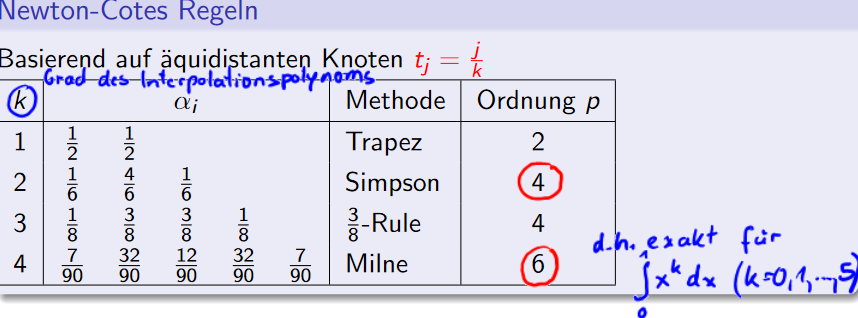
\includegraphics[scale=0.25]{./pic/NewtonCodesRegeln.png}
Falls $\alpha_{i} $ positiv. Integrationsregeln stabil; 
$ k \le 7 \& k =9 \Rightarrow $ positive Gewichte;
Bei halbierung der Intervalle \textbf{Nachfrage} vervierfacht or versechszehnfacht sich der Fehler?
\subsection{Ordnung Integrationsregel}
Eine Integrationsregel hat Ordnung p, wenn sie für Polynome vom Grad $\le$ p-1 exakte Werte liefert; $ T_{1} $ Ordnung 2 $\Rightarrow$ exakt für Polynome Grad $\le$ 1; 
Ordnung Newton-Cotes Regeln: mind. Ordnung k+1 (k: GRad des Interpolationspolynoms);
\textbf{Beweis der Ordnung:}
$ 1 = \int_{0}^{1} x^{0} dx \overset{!}{=} $; 
$ \frac{1}{2} = \int_{0}^{1} x dx \overset{!}{=} $; 
$ \frac{1}{3} = \int_{0}^{1} x^{2} \overset{!}{=} $; 
$ \frac{1}{4} = \int_{0}^{1} x^{3} \overset{!}{=} $; 
\subsection{Fehler Quadratur}
Für (globalen ) Fehler $ e_{In}  = \int_{a}^{b} f(x) dx -I_{n} $ einer Quadraturformel $I_{n} $ der Ordnung $ p$  auf $ [a,b] $ gilt: 
$ |e_{In} | = (b-a) h^{p}K|f^{ (p) } (\xi)| . \xi \in ]a,b[, h = \frac{ b-a }{ n}  $ \textbf{\&} 
$ |e_{In} | \le (b-a) h^{p} K \cdot max_{a \le x \le b} | f^{ (p) } (x) | $ ; 
\subsection{ Fehler $T_{n}$ }
Der Fehler ist proportional zu $ h^2 $; Eine Halbierung der Intervalllänge reduziert den Fehler um den Faktor $ \frac{1}{4} $; Ein Integral kann beliebig genau approx. werden, falls h entsprechend klein gewählt wird. \textbf{Aber} Rundungsfehler bei vielen Rechenoperationen, verschlechtert wieder das Ergebnis. Vorteil von Verfahren höherer Ordnung: Weniger Teilintervalle nötig.
$ |e_{T_n} | \le \frac{ h^2 }{12} (b-a) max_{a \le x \le b} | f^{''} (x) |, K =\frac{1}{12}, h = \frac{ b-a }{n} $

\subsection{Fehler $ S_{n} $}
Der Fehler ist proportional zu $ h^4 $; Eine Halbierung der Intervalllänge reduziert den Fehler um den Faktor $ \frac{1}{16} $;
$ | e_{Sn} | \le \frac{ h^{4} }{180} (b-a) max_{a \le x \le b} | f^{4} (x) |, h= \frac{(b-a)}{2n}, K = \frac{1}{180} $
\subsection{Grenzen NeCo}
viele äquidistante Knoten $\rightarrow$ Gewichte negativ $\rightarrow$ Verfahren instabil; 
geschlossene NeCoRe $\rightarrow$ Funktionsauswertung an RB $\rightarrow$ Problem mit Singularitäten.
größtmögliche Ordnung unerreichbar wegen äquidistanten Knoten; 
\textbf{Lösung:} 

\subsection{GauQua}